\subsubsection{Drivers and optocouplers}  \label{driver}

The control signal is generated by the control platform, which consists on a Plexim RTbox. In order to provide galvanic isolation between the converter and the control signal generator, optocouplers are used. The chosen optocoupler is the ACPL-P302. This optocoupler includes output signal circuitry which allows saving a pull-up or pull-down resistor. The integrated circuit (IC) is not an open collector device. Its main features might be seen at \ref{opto_features}.

\begin{table}[H]
	\centering
	\begin{tabular}{|p{4cm}|>{\centering}p{8cm}|}
		\hline
		\rowcolor{lightgray}\multicolumn{2}{|l|}{ \textbf{Maximum ratings}} \\ \hline
		Supply voltage & 35 [V]  \tabularnewline \hline
		Average input current & 25 [mA]  \tabularnewline \hline
		Peak output current & 0.4 [A]  \tabularnewline \hline
		\rowcolor{lightgray}\multicolumn{2}{|l|}{ \textbf{Other values of interest}} \\ \hline
		Input forward voltage & 1.5 [V]  \tabularnewline \hline
		Package & SSOIC6  \tabularnewline \hline
	\end{tabular}
	\caption{Optocoupler figures of meri
	\cite{opto_datasheet}.}
	\label{opto_features}
\end{table}

The signal from the optocoupler has to be amplified in order to drive the switches. The driver provides voltage amplification and current capability. The chosen IC to perform the task is NCP81074B. Find in table \ref{driver_features} its main features. 

\begin{table}[htbp]
	\centering
	\begin{tabular}{|p{6cm}|>{\centering}p{6cm}|}
		\hline
		\rowcolor{lightgray}\multicolumn{2}{|l|}{ \textbf{Maximum ratings}} \\ \hline
		Supply voltage & 24 [V]  \tabularnewline \hline
		Output current (pulse < 0.5 $\mu$s) & 10 [A]  \tabularnewline \hline		
		Reverse current (pulse < 1 $\mu$s) & 10 [A]  \tabularnewline \hline
		Input signal voltage & -6 to 24 [V]  \tabularnewline \hline
		\rowcolor{lightgray}\multicolumn{2}{|l|}{ \textbf{Other values of interest}} \\ \hline
		Output resistance & 0.4 [$\Omega$]  \tabularnewline \hline
		Package & SOIC8  \tabularnewline \hline
	\end{tabular}
	\caption{Driver figures of merit
		\cite{driver_datasheet}.}
	\label{driver_features}
\end{table}

The MOSFET is a voltage controlled device, the relationship between $V_{GS}$ and $V_{th}$ sets the drain to source maximum current, as seen in figure \ref{ids_vgs}\cite{mosfet_datasheet}.

\begin{figure}[H]
	\begin{center}
		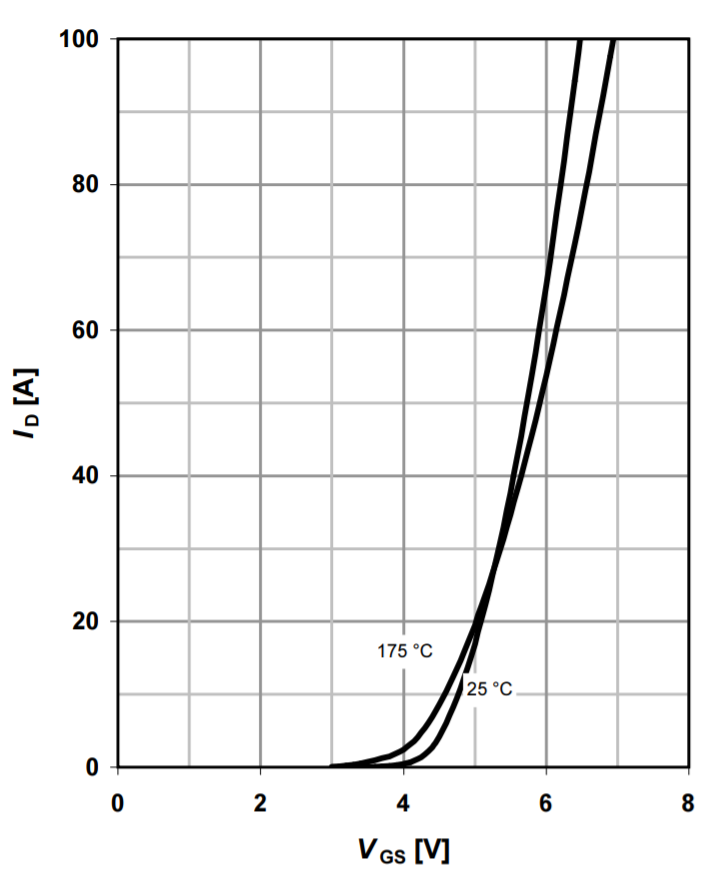
\includegraphics[width=0.5\textwidth]{../Pictures/P1/Component_sizing/ids_against_vgs.png}
		\caption{Drain to source current against gate to source voltage $(V_{DS} > 2 \cdot I_{D}\cdot R_{DSon})$.}
		\label{ids_vgs}
	\end{center}
\end{figure}


The dynamics of the switching can be modeled as a RC circuit, see figure \ref{mosfet_rc_gate}. Both $R_{driver \; out}$ and $R_{MOSFET}$ are directly obtained from the components' data sheets, while $R_{limiting}$ is the gate resistor which needs to be sized. $C_{iss}$ is also available in the MOSFET data sheet as input capacitance.



\begin{figure}[H]
	\begin{center}
		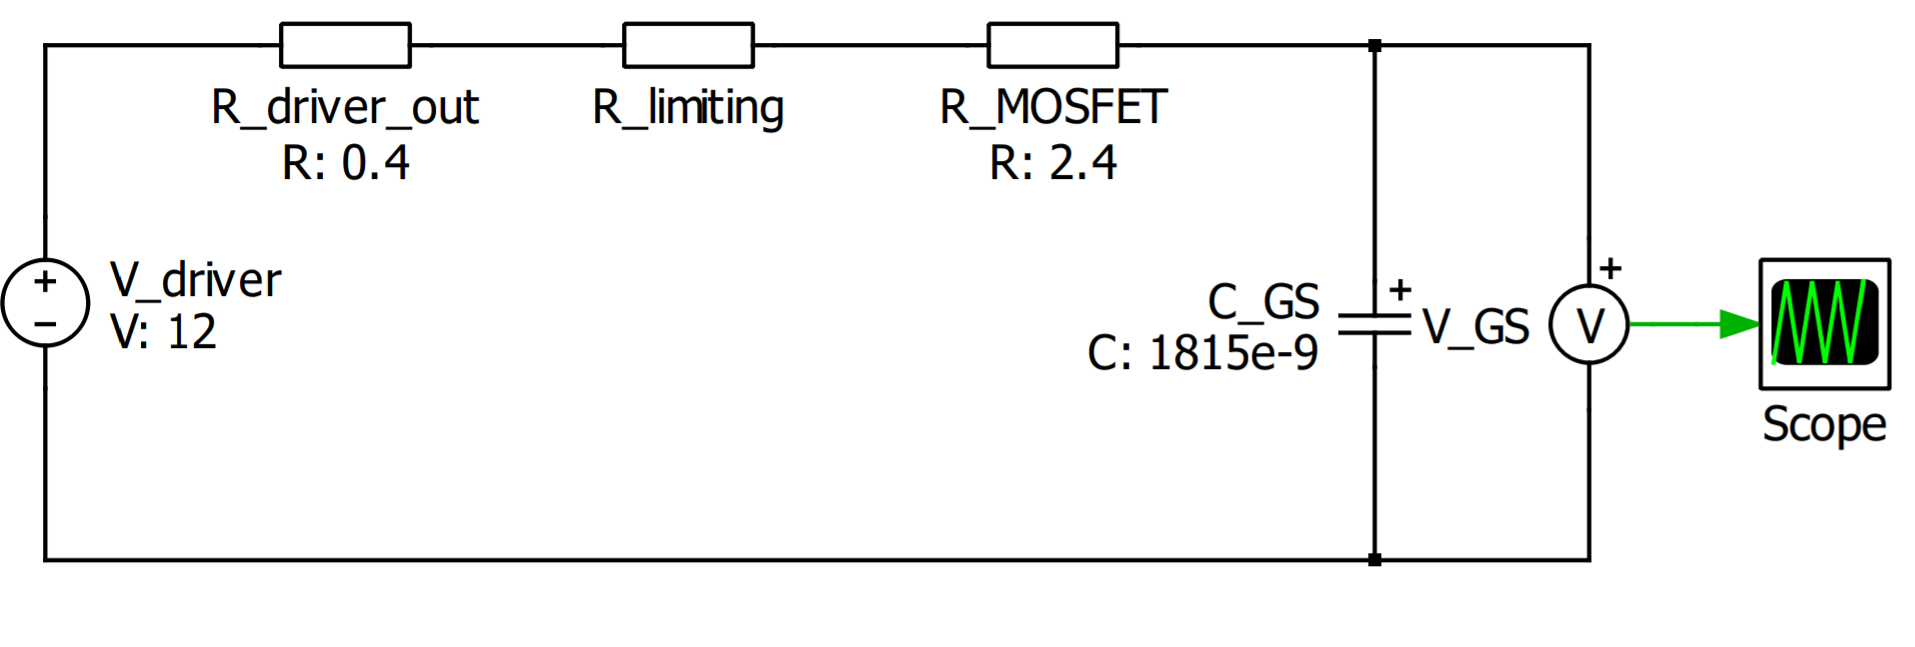
\includegraphics[width=0.8\textwidth]{../Pictures/P1/Component_sizing/driver_resistor_sizing.png}
		\caption{Simplified circuit used to model the MOSFET switching dynamics.}
		\label{mosfet_rc_gate}
	\end{center}	
\end{figure}

The time where the gate capacitor voltage reaches the threshold voltage produces a propagation delay from the driver output to the actual beginning of the MOSFET switching. In order to size the limiting resistor of the RC circuit, a time constraint was needed. This time constraint was arbitrarily set in relation with the switching frequency as described in equation \ref{time_constraint}. The 0.1\% constraint results in a limiting resistor of 20 $\Omega$. The average power dissipation, according to simulation, is 13 mW. This value is well under the power rating of the used SMD resistor with 1206 package, which is 250 mW. However the peak power dissipation was also considered, as it is relatively high. According to simulation, the peak is equal to 5.4 W, see figure \ref{gate_resistor_power_dissipation}. Although this value exceeds the resistor power rating, some manufacturers agree that the peak power dissipation in pulses shorter than 10 $\mu$s using 1206 resistors is 19 W \cite{pulse_withstanding_chip_resistors}, \cite{gate_driver_design_infineon}. Then the peak power dissipated shouldn't harm the component. Once the prototype is built, the thermal behaviour of the component is analysed with a thermal camera.

\begin{equation} \label{time_constraint}
t_{delay} = t\big\rvert_{V_{GS} = V_{th}} =\frac{T_{sw}}{1000} = 0.1 \% \;\; of \;\; T_{sw} = 20 \; ns
\end{equation}


\begin{figure}[H]
	\begin{center}
		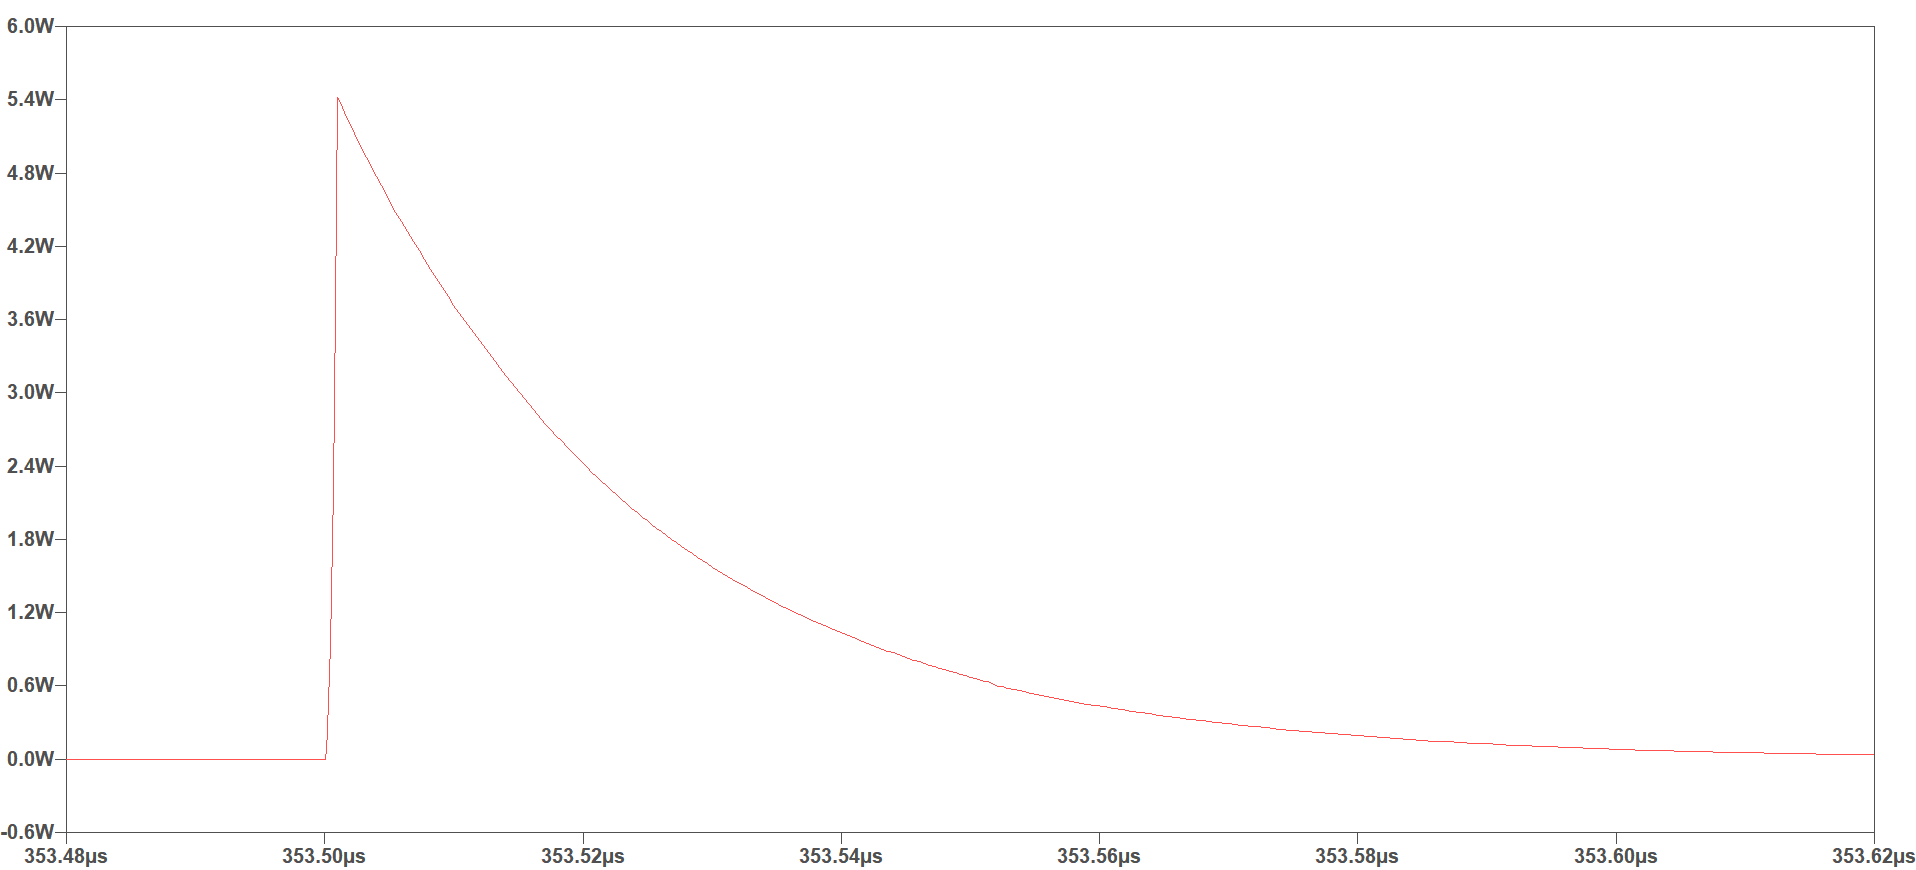
\includegraphics[width=\textwidth]{../Pictures/P1/Component_sizing/Gate_resistor_power_dissipation.png}
		\caption{Detail of the power dissipated at $R_{limiting}$ during MOSFET turn-on.}
		\label{gate_resistor_power_dissipation}
	\end{center}	
\end{figure}


The implemented topology has the peculiarity that two MOSFETs' sources are not directly connected to ground. As explained previously, it is the gate to source voltage that determines whether the transistor is conducting or not. In order to get a floating voltage in the high side drivers, one option is to have isolated supplies for those drivers. The ground of this isolated supplies will be tied to the low side MOSFET's drain. More explanation regarding the isolated supplies might be found at \ref{power_supplies}.

In case that the drivers were damaged, the residual voltage of the transistor's gate might become undefined, then, in order to ensure that the switch is off, a pull down resistor is added between the gate and the source of the transistor.
